\part{Week 6}
\chapter{Quantum circuits}
\section{Quantum algorithms}
Many interesting problems are impossible to solve on a classical computer, not because they're in principle insoluble, but because of the astronomical amount of resources they'd need. Quantum computing promises to enable feasible algorithms which would require unreasonably high resources for a solution on a classical computer.

As we've discussed before, two broad classes of quantum algorithms exist now, first is based on Shor's \textit{Quantum fourier transform} which provides \textit{exponential} speedup. Second is based on Grover's algorithm for performing \textit{quantum searching} which provides \textit{quadratic} speedup. Few main applications are listed in this figure
\begin{figure}[H]
    \centering
    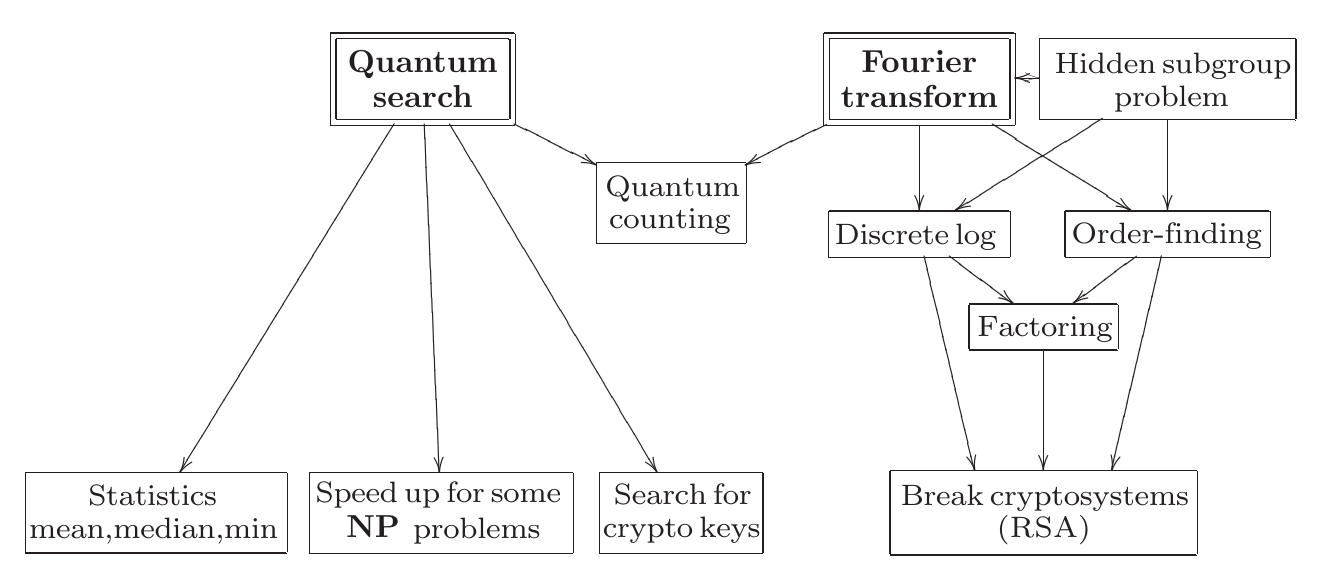
\includegraphics[width=0.9\textwidth]{images/quantum_algorithms.png}
    \caption{Main quantum algorithms with their applications and relationships.}
    \label{fig:quantum-algorithms}
\end{figure}

\section{Single qubit operations}
A single qubit is the simplest quantum system. We already know few important things like norm of the state is 1, operations on it are defined by unitary matrices etc. Few important gates/ operations are Pauli matrices ($I$, $X$, $Y$, $Z$) which we know. Three other important quantum gates are Hadamard gate ($H$), phase gate ($S$), and $\pi/8$ gate ($T$):
\begin{equation}
    H = \frac{1}{\sqrt{2}}\begin{bmatrix}
        1 & 1 \\ 1 & -1
    \end{bmatrix};
    \ \ \ 
    S = \begin{bmatrix}
        1 & 0 \\ 0 & i
    \end{bmatrix};
    \ \ \ 
    T = \begin{bmatrix}
        1 & 0 \\ 0 & \exp{(i\pi/4)}
    \end{bmatrix}.
\end{equation}
Few useful facts are $H = (X+Z)/\sqrt{2}$ and $S=T^2$, $T$ is known as $\pi/8$ gate instead of $\pi/4$ because it's equal to a gate with diagonal $\exp{(\pm \pi/8)}$ upto a global phase factor:
\begin{equation}
    T = \exp{(i\pi/8)}\begin{bmatrix}
        \exp{(-i\pi/8)  } & 0 \\ 0 & \exp{(i\pi/8)}
    \end{bmatrix}
\end{equation}
Also, in \textit{Bloch sphere} representation, the state $a\qo+b\qi$ can be represented as a point $(\theta, \varphi)$ where $a=\cos{(\theta/2)}$ and $b=e^{i\varphi}\sin{(\theta/2)}$, and the Bloch vector is $(\cos{\varphi}\sin{\theta}, \sin{\varphi}\sin{\theta}, \\ \cos{\theta})$.

Pauli matrices give rise to useful matrices when exponentiated, the \textit{rotation operators} about $\hat{x}$, $\hat{y}$ and $\hat{z}$ axes, defined by equations
\begin{align}
    % 1
    R_x(\theta) & \equiv e^{-i\theta X/2} = \cos{\frac{\theta}{2}}I - i\sin{\frac{\theta}{2}}X = \begin{bmatrix}
        \cos{\frac{\theta}{2}} & -i\sin{\frac{\theta}{2}} \\
        -i\sin{\frac{\theta}{2}} & \cos{\frac{\theta}{2}} 
    \end{bmatrix} \\
    % 2
    R_y(\theta) & \equiv e^{-i\theta Y/2} = \cos{\frac{\theta}{2}}I - i\sin{\frac{\theta}{2}}Y = \begin{bmatrix}
        \cos{\frac{\theta}{2}} & -\sin{\frac{\theta}{2}} \\
        \sin{\frac{\theta}{2}} & \cos{\frac{\theta}{2}}
    \end{bmatrix} \\
    % 3
    R_z(\theta) & \equiv e^{-i\theta Z/2} = \cos{\frac{\theta}{2}}I - i\sin{\frac{\theta}{2}}Z = \begin{bmatrix}
        e^{-i\theta/2} & 0 \\
        0 & e^{i\theta/2}
    \end{bmatrix} .
    \end{align}
this is because if $x\in \mathbb{R}$ and $A^2=I$, then $e^{iAx}=\cos{x}I+i\sin{x}A$. If $\hat{n}=(n_x,n_y,n_z)$ is real unit vector in three dimensions then generalize the rotation by $\theta$ about $\hat{n}$ by the equation
\begin{equation}
    R_{\hat{n}}(\theta) = e^{-i\theta \hat{n}\cdot \Vec{\sigma}/2} = \cos{\left( \frac{\theta}{2} \right)}I - \sin{\left( \frac{\theta}{2} \right)}(n_xX+n_yY+n_zZ),
\end{equation}
where $\Vec{\sigma}$ denotes the three component vector $(X, Y, Z)$ of Pauli matrices. A nice fact is that any unitary operator on a single qubit can be written as $U=e^{i\alpha}R_{\hat{n}}(\theta)$ for some $\alpha$, $\hat{n}$ and $\theta$. More generally

\begin{theorem}[\textbf{Z-Y decomposition for a single qubit}]
    Suppose $U$ is a unitary operation on a single qubit. Then there exist real numbers $\alpha$, $\beta$, $\gamma$, $\delta$ such that
    \begin{equation}
        U = e^{i\alpha}R_z(\beta)R_y(\gamma)R_z(\delta)
    \end{equation}
\end{theorem}
In general $z$ and $y$ can be replaced by any non-parallel real unit vectors $\hat{m}$ and $\hat{n}$. Also, this leads to a mysterious corollary, which'll be useful later.
\begin{corollary}
    Suppose $U$ is a unitary gate on a single qubit. Then there exist unitary operators $A$, $B$, and $C$ on a single qubit such that $ABC=I$ and $U=e^{i\alpha}AXBXC$, where $\alpha$ is some overall phase factor.
\end{corollary}
Here are few useful circuit identities:
\begin{equation}
    HXH = Z;\ HYH = -Y;\ HZH = X.
\end{equation}
also, $HTH=R_x(\pi/4)$. To recap things here are few quantum circuit symbols
\begin{figure}[H]
    \centering
    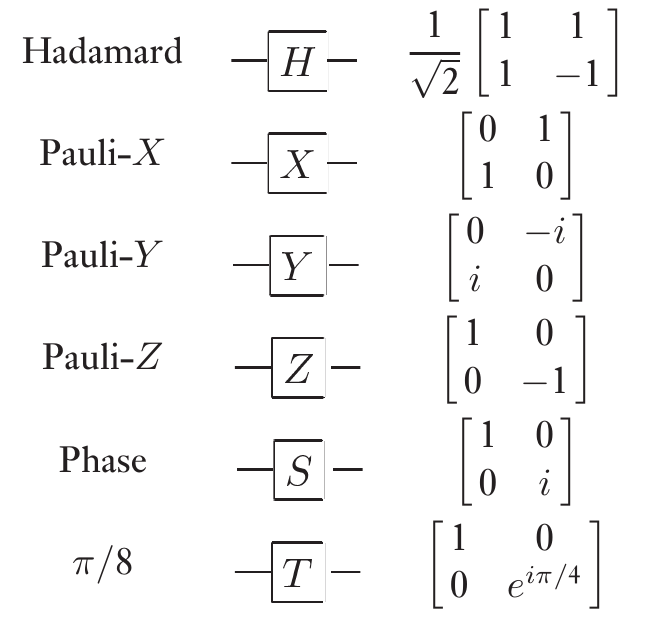
\includegraphics[width=0.4\textwidth]{images/circuit_symbols.png}
    \caption{Names, symbols and unitary matrices for commonly used quantum gates.}
    \label{fig:circuit-symbols}
\end{figure}
\section{Controlled operations}
`If $A$ is true, then do $B$' is the most useful and basic controlled operation in both classical and quantum computation. An example is \textsc{cnot} gate in quantum computation, which does $\ket{c}\ket{t}\rightarrow \ket{c}\ket{t\oplus c}$ where $\ket{c}$ is control qubit and $\ket{t}$ the target qubit. If $\ket{c}$ is in state $\qo$ nothing happens to target qubits, else if it's in $\qi$ $\ket{t}$ is flipped. A general thing for this is \textit{controlled-U} gate, which does $\ket{c}\ket{t}\rightarrow \ket{c}U^c\ket{t}$, where $U$ is a unitary operation. In the computational basis $\ket{\text{control, target}}$, the matrix representation of \textsc{cnot} gate is
\begin{equation}
    \begin{bmatrix}
        1 & 0 & 0 & 0 \\
        0 & 1 & 0 & 0 \\
        0 & 0 & 0 & 1 \\
        0 & 0 & 1 & 0
    \end{bmatrix}.
\end{equation}

To develop \textit{controlled-U} gate for arbitrary $U$, we'll use $U=e^{i\alpha}AXBXC$. To apply the controlled phase shift $\exp{(i\alpha)}$, we use a circuit containing a single qubit gate as shown
\begin{figure}[H]
    \centering
    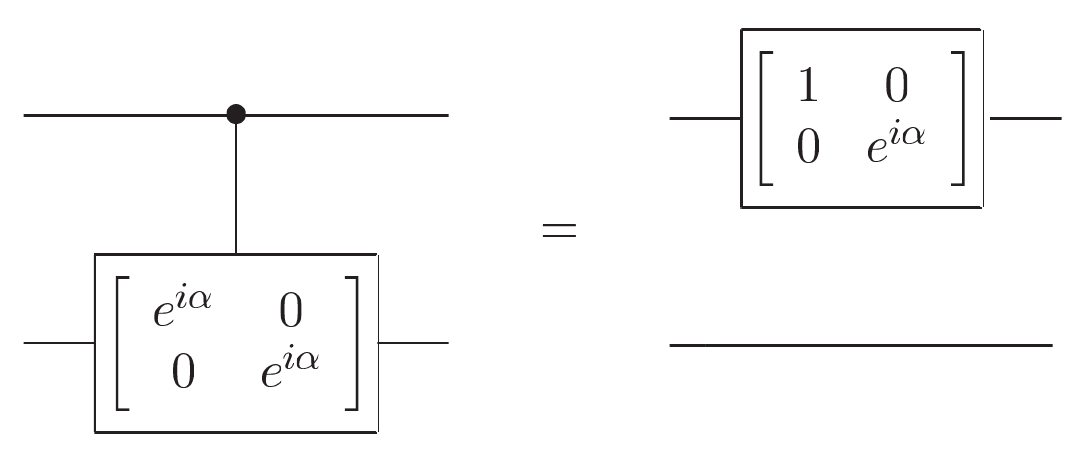
\includegraphics[width=0.5\textwidth]{images/phase_shift_circuit.png}
    \caption{Controlled phase shift gate and an equivalent circuit for two qubits.}
    \label{fig:phase-shift-circuit}
\end{figure}

To complete the gate we use the circuit \ref{fig:controlled-u-circuit}. This works because if control qubit is set to $\qo$ then nothing happens at \textsc{cnot} gates and $ABC=I$ is applied which does nothing, if control qubit is $\qi$ then $e^{i\alpha}AXBXC$ is applied, thus $U$ is applied. 
\begin{figure}[H]
    \centering
    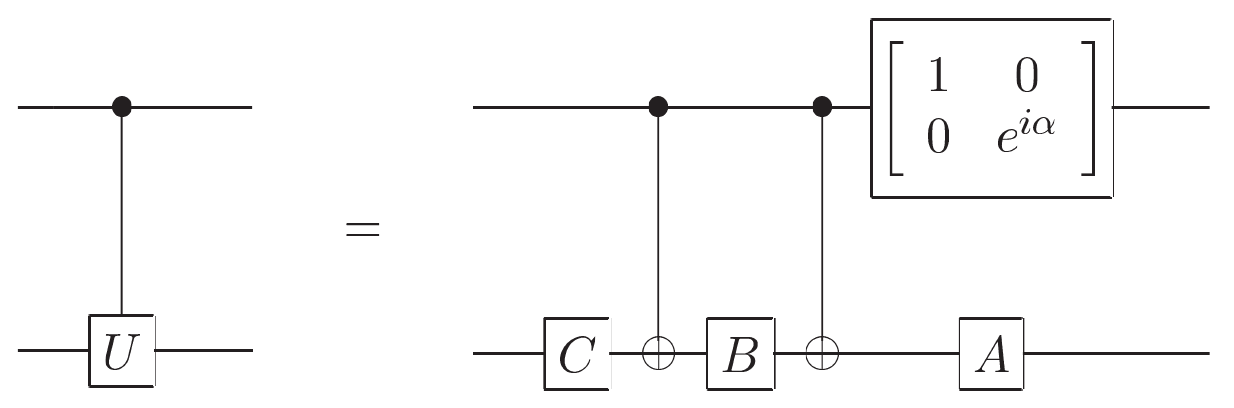
\includegraphics[width=0.7\textwidth]{images/controlled_u_circuit.png}
    \caption{\textit{controlled-U} circuit, $\alpha$, $A$, $B$, $C$ satisfy $U=e^{i\alpha}AXBXC$ and $ABC=I$}
    \label{fig:controlled-u-circuit}
\end{figure}

To use conditioning on multiple-qubits, suppose we have $n+k$ qubits, and $U$ is a $k$ bit operator. Then the controlled operatioin $C^n(U)$ by the equation
\begin{equation}
    C^n(U)\ket{x_1x_2\dots x_n}\qv = \ket{x_1x_2\dots x_n}U^{x_1x_2\dots x_n}\qv
\end{equation}
where $x_1x_2\dots x_n$ means product of those bits. It means operation $U$ is applied on last $k$ qubits if all of the first $n$ qubits are $\qi$. We'd assume $k=1$, for $k\geq2$ we don't yet know how to perform $k$ arbitrary operations at once.
\begin{figure}[H]
    \centering
    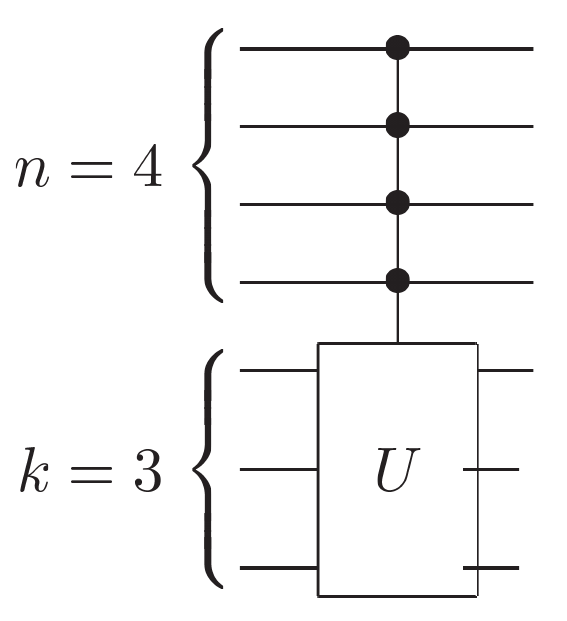
\includegraphics[width=0.4\textwidth]{images/multi_qubit_operation_circuit.png}
    \caption{$C^n(U)$ operation for $n=4$ and $k=3$.}
    \label{fig:multi-qubit-operation}
\end{figure}